\chapter{User Study Results} \label{App:User Study Results}

\begin{preamble}
	An appendix detailing results from the user study.
\end{preamble}

\begin{landscape}

\begin{figure}[h]
\begin{center}
	\vspace{-10pt}
	\makebox[\textwidth]{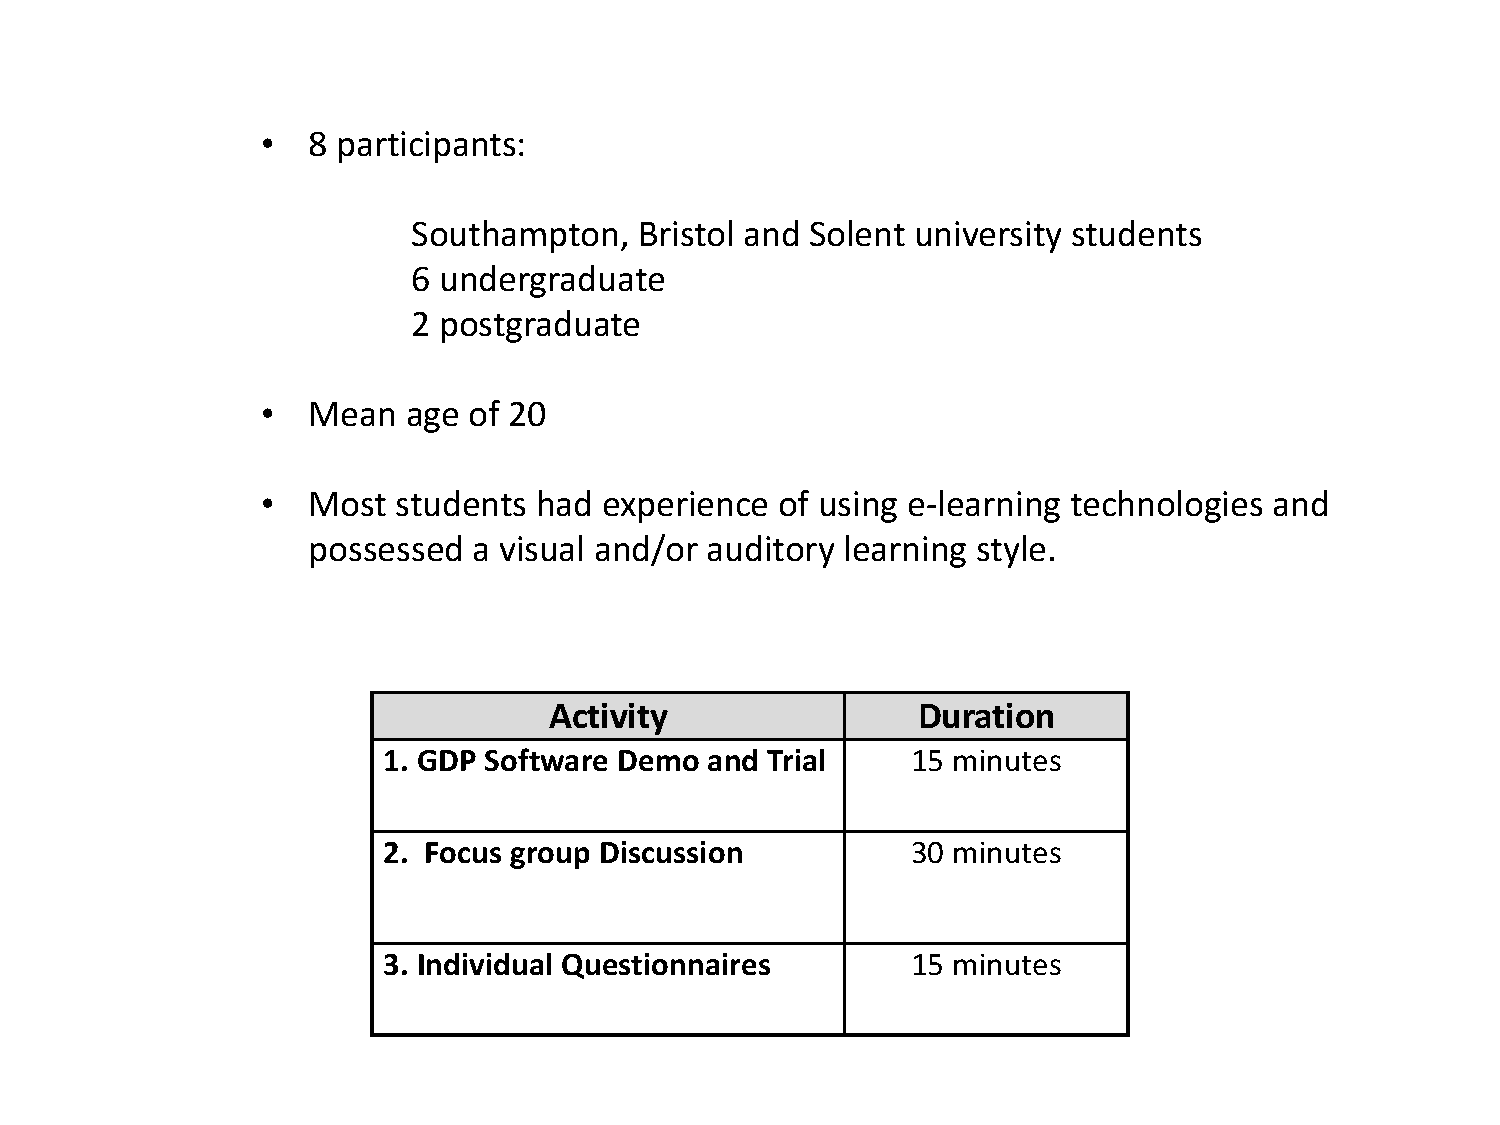
\includegraphics[width=18cm, page=1]{UserStudyReport.pdf}}
\end{center}
\caption{\label{Figure:User study presentation page 1} Page 1 of user study presentation}
\end{figure}

\begin{figure}[h]
\begin{center}
	\vspace{-10pt}
	\makebox[\textwidth]{\includegraphics[width=18cm, page=2]{UserStudyReport.pdf}}
\end{center}
\caption{\label{Figure:User study presentation page 2} Page 2 of user study presentation}
\end{figure}

\begin{figure}[h]
\begin{center}
	\vspace{-10pt}
	\makebox[\textwidth]{\includegraphics[width=18cm, page=3]{UserStudyReport.pdf}}
\end{center}
\caption{\label{Figure:User study presentation page 3} Page 3 of user study presentation}
\end{figure}

\begin{figure}[h]
\begin{center}
	\vspace{-10pt}
	\makebox[\textwidth]{\includegraphics[width=18cm, page=4]{UserStudyReport.pdf}}
\end{center}
\caption{\label{Figure:User study presentation page 4} Page 4 of user study presentation}
\end{figure}

\begin{figure}[h]
\begin{center}
	\vspace{-10pt}
	\makebox[\textwidth]{\includegraphics[width=18cm, page=5]{UserStudyReport.pdf}}
\end{center}
\caption{\label{Figure:User study presentation page 5} Page 5 of user study presentation}
\end{figure}

\end {landscape}

These results were presenting during a client meeting by Shameem, during this we reviewed some of the requirements that were apparent after the user study.

On reviewing requirements with the customer FR1 and FR2 was already implemented but needed some more expansive user code. FR3 and FR4 was considered out of scope by the client. FR5, FR6, and NFR6 were considered a Synote addition that would fit better in Synote. NFR1, NFR2, NFR4, and NFR5 were already requirements given by the client so no changes were needed. NFR3 was considered to be implemented but the client recommended prioritising on the core features before working on this. 
